\documentclass{osmscience}

% Add bibliography file here (class does not add it)
\addbibresource{bibliography.bib}

\title{From centroid to entrance: quantifying POI access-location error worldwide and on large Quebec sites}
\author[1,*]{Pierre-Léo Bourbonnais}
\author[1]{Yannick Brosseau}
\author[1]{Catherine Morency}
\affil[1]{
    Polytechnique Montréal, Montréal, Canada\\
    \href{mailto:leo.bourbonnais@polymtl.ca}{\underline{leo.bourbonnais@polymtl.ca}}
}

% DOI Information (to be filled after Zenodo upload)
\proceedingsDOI{10.5281/zenodo.21473694}
\proceedingsFirstPage{1} % TODO
\date{}

\begin{document}
\maketitle

\vspace{1em}

Points of interest (POIs) serve as origins and destinations when estimating travel demand and modelling mobility behaviour. Common practice approximates locations by area or building centroids, both in GIS-based service-area studies and in POI quality assessments \cite{Gutierrez2008, Biba2010, Klinkhardt2023}. This mirrors, at the site scale, the zone-centroid representation at the core of operational travel demand models, in which all trip ends collapse to traffic-zone centroids and transit walk access and egress times are computed from them \cite{Miller2021}, and where the placement of the centroid connectors themselves measurably distorts travel times \cite{Qian2012}. On small single-purpose buildings this substitution is harmless; on larger and multi-building sites the centroid can misrepresent the access point by hundreds of metres, occasionally kilometres. OpenStreetMap (OSM) can encode true access points through the \texttt{entrance=*} tag (\texttt{main}, \texttt{customers}, \texttt{home}, \ldots) and the routing-oriented \texttt{routing:entrance=*} tag, but these tags remain sparsely mapped: Hu et al.\ found only about sixty tagged buildings in an entire London extract \cite{Hu2021}. We stress that the magnitude of this error is not equally relevant to every transport model. Regional four-step or aggregate demand models are insensitive to sub-100\,m displacements. The error matters for very large areas, and for models and services in which the stop-to-door or curb-to-door segment is a first-class quantity: transit catchment and walking-access estimation \cite{Gutierrez2008, ElGeneidy2014}, wheelchair and paratransit routing \cite{Neis2014}, and curbside pick-up/drop-off placement for ride-hailing and autonomous vehicles \cite{Hunter2024, Wang2025}. Our prior validation of 1{,}034 POIs from five Québec household travel surveys found median positional errors around 20\,m across OSM, Overture Maps, the Québec property registry and Google Places, with long error tails dominated by university campuses and hospital complexes \cite{Bourbonnais2026}. The present study complements it with two empirical cohorts processed through a single pipeline: a worldwide random sample of POIs, and a targeted regional selection of large Québec POIs where the centroid proxy is expected to fail hardest.

The worldwide cohort is drawn by tessellating the globe into $10\times10$\,km cells and sampling cells with probability proportional to an equal weight of population (GHS-POP) and built volume (GHS-BUILT-V); the built-volume term prevents low-residential but high industrial, institutional, leisure or commercial activity from being under-sampled. Within kept cells, POIs are selected at random from OSM features. The targeted Québec cohort covers every registered university campus in the province (57 sites), split between large and small campuses (satellite or single-building sites), together with the 10 largest hospitals (by bed count), 18 of the largest shopping centres, the 10 most visited national parks (SÉPAQ) and the 3 international airports (YUL, YQB, YHU). For every POI in either cohort, reference main entrances are established manually from aerial imagery and open and proprietary street-level imagery (Mapillary, KartaView, Panoramax, Google Street View, Baidu Panorama), complemented where available by architectural or wayfinding plans; the analyst inspects the site perimeter and only accepts an entrance when at least one recent source shows it unambiguously. This manual protocol is deliberate: it produces reference-quality ground truth against which scalable automated approaches \cite{Hu2021} can later be evaluated, and it is not proposed as a production method. In the worldwide cohort, 51 of 167 randomly drawn POIs (30.5\,\%) were rejected because no aerial or street-level imagery allowed confident entrance location, or in a few cases because the POI no longer exists; rejections concentrate in specific countries (e.g.\ 10 in India, 4 in Nigeria), so the rejection rate is itself a measurement of the heterogeneity of open imagery and OSM coverage worldwide. For each accepted POI, the analyst draws and persists shortest paths along the walking network from two anchors---the reference centroid and the main entrance---towards the same targets: the nearest publicly drivable road and the nearest known transit stop when available. The reference centroid deliberately mirrors current practice: for POI classes conventionally mapped in OSM as areas (universities, schools, colleges, hospitals, parks, \ldots) it is the centroid of the area---which is also the point a geocoder such as Nominatim returns by default, as searching for a university yields the campus area and its centroid. For classes conventionally mapped as buildings, or as nodes placed on a building, it is the centroid of the building. Our measured differences therefore quantify the error currently incurred when routing to a geocoded or centroid-collapsed POI. Nominatim has recently begun exposing \texttt{entrance=*} and \texttt{routing:entrance=*} nodes as optional output, but its default result point remains the centroid \cite{Nominatim2025}. Each polyline stores its geodesic length, walking duration at 5\,km/h, purpose and anchor class. Two derived quantities drive the analysis: the network walking distance from centroid to main entrance, and, for each (centroid, main-entrance) pair aimed at the same target family, whether the two walks end more than 10\,m apart---that is, whether the centroid proxy identifies a \emph{different} access road point or a \emph{different} transit stop than the true entrance. During the analysis, missing entrances and missing pedestrian-access geometry were added to OSM for every processed POI (234 changesets); all edits carry the \texttt{\#StateOfTheMap2026} and \texttt{\#EntranceAnalysis} changeset hashtags and are therefore fully traceable.

The Rust/PostGIS/React pipeline, the sampled POI lists and all persisted measurements are released openly at \url{https://github.com/chairemobilite/stateofthemap2026} (drafting and parts of the pipeline were assisted by Anthropic Claude Opus 4.8 and Fable 5; all measurements, data, methods and findings remain the authors').

Across the 116 accepted worldwide POIs, the network distance from centroid to main entrance is modest for the typical POI---median 28\,m, with 79.3\,\% of POIs within 100\,m---but the distribution is heavily right-skewed: 20.7\,\% of POIs exceed 100\,m, 9.5\,\% exceed 250\,m and 2.6\,\% reach 1\,km or more, up to 14.9\,km for the Mount Kenya National Reserve, whose area centroid lies deep inside the massif. Pairing walks to identical targets shows the same asymmetry: towards the nearest drivable road the centroid-minus-entrance difference has a median of 14\,m but a maximum of 5{,}094\,m ($n=116$), and towards the nearest transit stop a median of 26\,m but a maximum of 439\,m ($n=32$). Beyond magnitude, the proxy also produces \emph{topological} errors: for 30 of the 116 road pairs (26\,\%) the walk from the centroid ends on a different road access point than the walk from the entrance, and 2 of the 32 transit pairs select a different stop. Notably, 84 of the 116 worldwide POIs (72\,\%) had no nearby transit stop in either of the two sources used to locate stops, OSM and Google Maps. Stop data from these sources were available almost everywhere except China; outside China, the absence of a measurable stop can therefore be read as a genuine absence of regular transit service within walking range of the POI, whereas for the 27 Chinese POIs of the sample the absence remains inconclusive.

The targeted Québec cohort shows that these tail behaviours become the norm as site scale grows, as summarized in \figref{fig:results}. On the 39 small university campuses, the median centroid-to-entrance network distance is 102\,m, 51\,\% of sites exceed 100\,m, and the centroid selects a different road access point on 22 of 39 pairs and a different transit stop on 5 of 29 pairs. Shopping centres and hospitals sit further along the gradient: 16 of 18 shopping centres and 9 of 10 hospitals lie beyond 100\,m (7 of 10 hospitals beyond 250\,m), with divergent road access points on 11 of 18 and 9 of 10 pairs and divergent transit stops on 8 of 18 and 6 of 10 pairs, respectively. On the 18 large campuses the failure is nearly systematic: median 304.5\,m (maximum 2{,}806\,m), 89\,\% of sites beyond 100\,m and 78\,\% beyond 250\,m, a different road access point on 16 of 18 pairs (89\,\%) and a different transit stop on 12 of 18 pairs (67\,\%). At territorial scale the proxy collapses entirely: all 10 national parks and all 3 airports lie at 1\,km or more from their centroid to their main entrance (parks: median 8.7\,km, up to 46\,km), with divergent road access points on 9 of 10 park pairs and 3 of 3 airport pairs (8 of the 10 parks have no transit stop at all). Reading the cohorts together yields a clean monotone gradient with site scale---POIs beyond 100\,m rise from 20.7\,\% (random worldwide) through 51\,\% (small campuses), 89--90\,\% (shopping centres, large campuses, hospitals) to 100\,\% (national parks, airports), and divergent road access points from 26\,\% to 100\,\%. In other words, for the typical randomly drawn POI the centroid proxy is indeed benign, consistent with the uncertainty margins of aggregate models; but precisely on the large trip generators---campuses, shopping centres, hospitals, parks, airports---the proxy does not merely add metres, it routes towards the wrong access road and assigns the wrong transit stop in a majority of cases, an error class that no error margin absorbs.

\begin{figure}[ht]
    \centering
    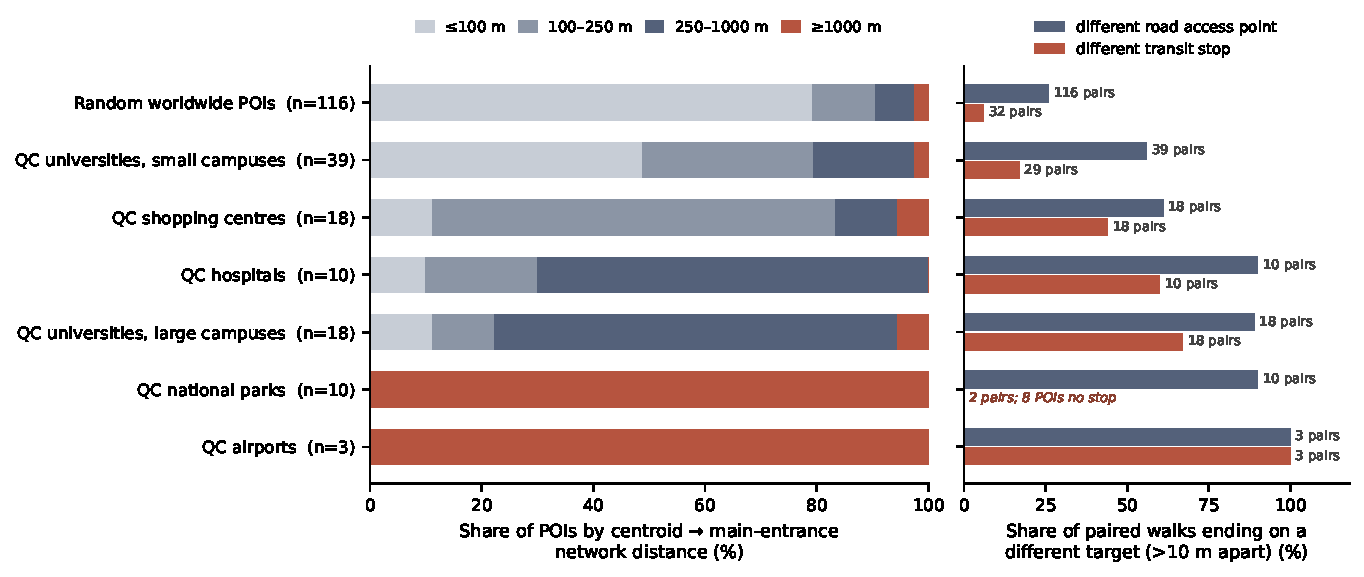
\includegraphics[width=0.95\textwidth]{figure_results}
    \caption{Left: share of POIs by network walking distance from centroid to main entrance, by cohort (POI counts from exact bin counts). Right: share of paired walks towards the same target whose endpoints land more than 10\,m apart, i.e.\ the centroid identifies a different road access point or transit stop than the main entrance; annotations give the number of measurable pairs. Cohorts ordered by severity; the Mount Kenya extreme belongs to the worldwide cohort.}
    \label{fig:results}
\end{figure}

These results carry two implications. First, entrance-level information is not a luxury refinement of OSM data but a prerequisite for pedestrian-scale accessibility work on large sites (car accessibility is also almost always incorrect for large areas like national parks), and the \texttt{entrance=*} tag deserves mapping attention proportional to site footprint; the measured gradient offers a simple prioritization rule. Second, the 30.5\,\% rejection rate of the worldwide random draw quantifies how unevenly the imagery and data needed for entrance verification are distributed across the globe; a worldwide sampling frame is not a weakness but the only way to observe this heterogeneity. Ongoing work extends the targeted Québec cohort to further sites and categories of large trip generators and will contrast field-validated survey destinations \cite{Bourbonnais2026} with both centroid and entrance anchors.

\printbibliography

\end{document}